\chapter{Analisi sperimentale}
\label{cha:NTPsec} \label{cha:NTPsec}

Il presente capitolo è dedicato all’analisi dei dati raccolti per il demone
\textbf{NTPsec}, con l’obiettivo di valutarne il comportamento al variare delle
condizioni di rete introdotte nei tre scenari sperimentali. L’attenzione è rivolta
all’esame delle principali metriche di sincronizzazione temporale osservate durante
la fase di testing, al fine di evidenziare l’eventuale impatto del progressivo
incremento degli impairment di rete sulla stabilità del sistema e sulla qualità
del processo di sincronizzazione.

L’analisi è organizzata per metrica. Per ciascuna grandezza considerata viene condotto
un confronto sistematico tra i tre scenari sperimentali definiti in precedenza,
corrispondenti a differenti livelli di degrado della rete (\texttt{low}, \texttt{medium},
\texttt{high}). Tale confronto si basa sull’osservazione dei dati raccolti e
sulla loro rappresentazione grafica, con lo scopo di mettere in evidenza eventuali
variazioni nel comportamento del demone in termini di accuratezza della sincronizzazione,
variabilità delle misurazioni e dinamica di convergenza.

\vspace{0,2 cm}
\begin{table}[h]
  \centering
  \caption{Matrice di scenario - fase 3 (topologia T2 + NETEM)}
  \begin{tabular}{|c|c|c|c|c|c|}
    \hline
    \textbf{Scenario} & \textbf{Delay} & \textbf{Jitter} & \textbf{Loss} & \textbf{Reorder} & \textbf{Rate Limit} \\
    \hline
    LOW               & 5 ms           & 1 ms            & 0.1\%         & 1\%              & 50 Mbit             \\
    \hline
    MEDIUM            & 15 ms          & 5 ms            & 0.5\%         & 5\%              & 20 Mbit             \\
    \hline
    HIGH              & 60 ms          & 20 ms           & 10\%          & 20\%             & 5 Mbit              \\
    \hline
  \end{tabular}
  \label{tab:scenario_matrix}
\end{table}
\section{\texttt{NTPsec}}

Nel caso di \textbf{NTPsec}, l’analisi si concentra su tre metriche principali:
\textbf{delay}, \textbf{jitter} e \textbf{offset}. Tali grandezze consentono di caratterizzare,
rispettivamente, il tempo di propagazione dei pacchetti NTP, la variabilità
temporale delle misurazioni e lo scostamento tra il clock locale e il clock di
riferimento. La loro evoluzione nei diversi scenari permette quindi di valutare la
robustezza del demone rispetto al degrado delle condizioni di rete e di analizzare
la qualità del processo di sincronizzazione in termini sia di stabilità sia di accuratezza.

I dati oggetto dell’analisi sono stati raccolti secondo la metodologia sperimentale
illustrata nei capitoli precedenti. In questa sede, pertanto, non vengono
ripresi gli aspetti relativi alla configurazione dell’ambiente di prova o alla
disposizione della topologia, ma si assume come riferimento l’insieme delle misurazioni
già ottenute per ciascuna metrica e per ciascuno scenario di rete. Nel caso
specifico di \textbf{NTPsec}, le misurazioni considerate sono state rilevate sui
nodi \texttt{clientntp} e \texttt{boundary} della topologia, in coerenza con il ruolo
da essi ricoperto nel processo di sincronizzazione.

Ciascuna sezione seguente è quindi dedicata a una singola metrica e presenta,
per i tre scenari sperimentali, i risultati osservati e il relativo confronto interpretativo,
con l’obiettivo di individuare eventuali differenze significative tra le
condizioni di rete considerate e valutarne gli effetti sul comportamento del
demone.

\newpage
\subsection{\texttt{clientntp}}
L'analisi condotta sul nodo \texttt{clientntp} è caratterizzata da uno stato di inizializzazione,
identificato da \texttt{refid=.INIT.}, \texttt{stratum=16}, \texttt{selected=False}
e \texttt{reach=0}. Tale intervallo non rappresenta il regime operativo della sincronizzazione
e non viene quindi considerato nel confronto tra scenari, che viene invece
condotto a partire dal primo campione valido, corrispondente in tutti i casi a circa
601 secondi di tempo relativo.
\subsubsection{Analisi metrica: \texttt{delay}}
\begin{figure}[H]
  \centering

  \begin{subfigure}
    {0.32\textwidth}
    \centering
    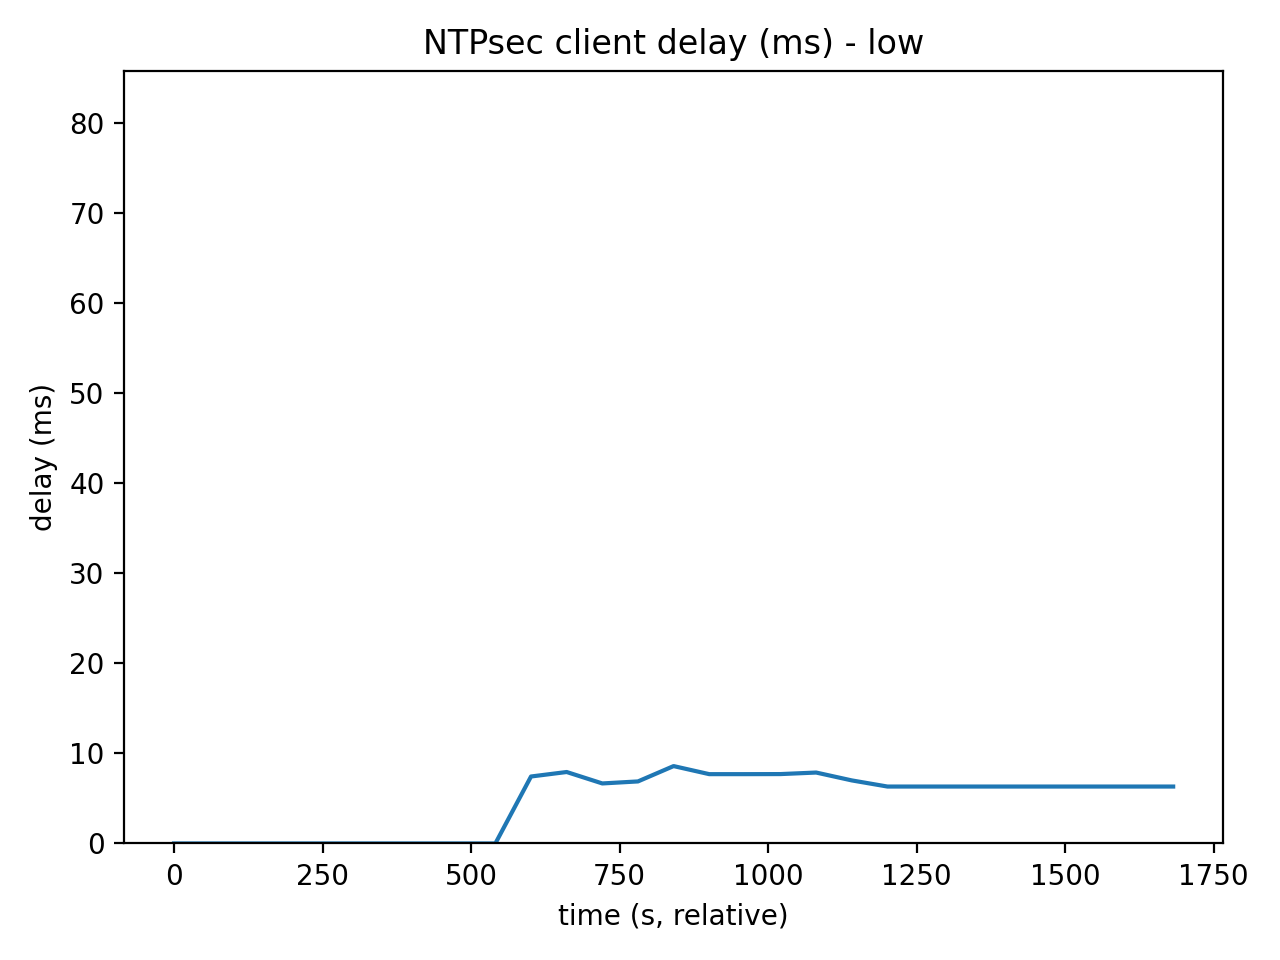
\includegraphics[width=\linewidth]{
      images/data_plots/plots_ntpsec/ntpsec_client_low_delay_ms.png
    }
    \caption{Scenario LOW}
  \end{subfigure}
  \hfill
  \begin{subfigure}
    {0.32\textwidth}
    \centering
    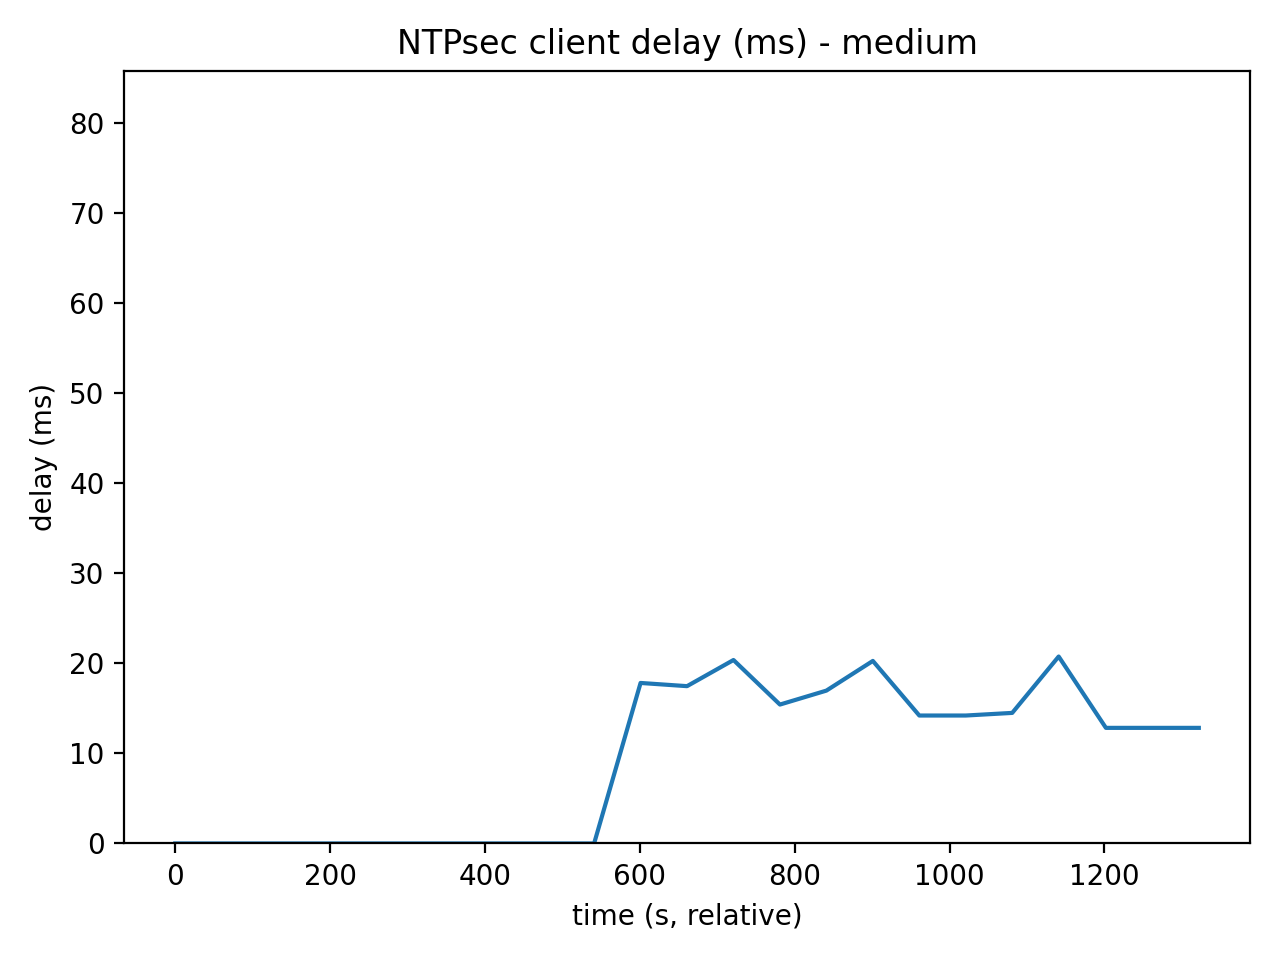
\includegraphics[width=\linewidth]{
      images/data_plots/plots_ntpsec/ntpsec_client_medium_delay_ms.png
    }
    \caption{Scenario MEDIUM}
  \end{subfigure}
  \hfill
  \begin{subfigure}
    {0.32\textwidth}
    \centering
    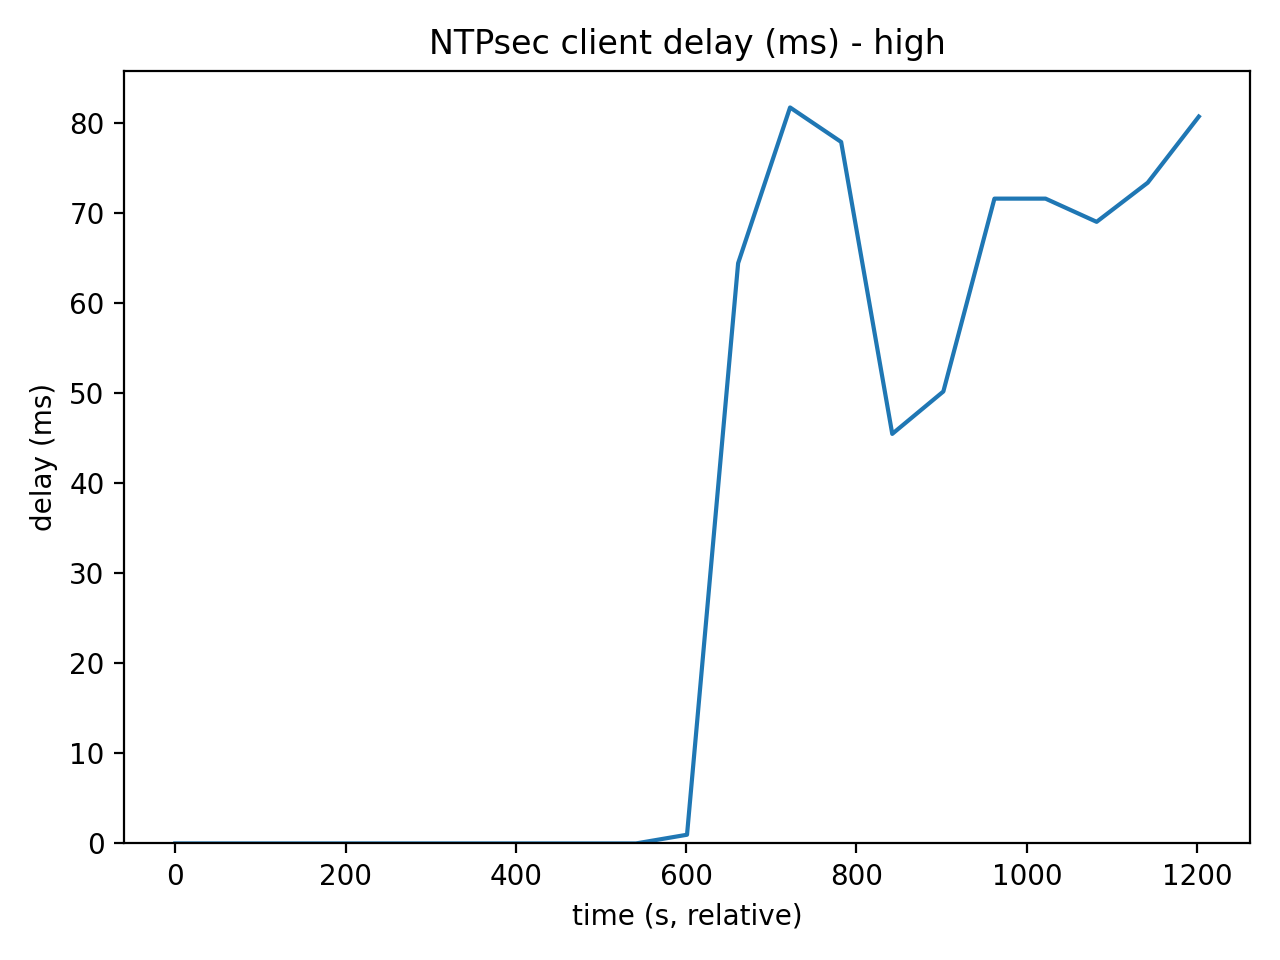
\includegraphics[width=\linewidth]{
      images/data_plots/plots_ntpsec/ntpsec_client_high_delay_ms.png
    }
    \caption{Scenario HIGH}
  \end{subfigure}

  \caption{Comparazione della performance - nodo: \texttt{clientntp}}
  \label{fig:scenario_comparison}
\end{figure}

L’analisi del \textbf{delay} misurato sul nodo \texttt{clientntp} per il demone \textbf{NTPsec}
evidenzia una dipendenza marcata dal livello di impairment introdotto nei tre
scenari sperimentali. Il risultato mette in evidenzia un consistente e progressivo
degrado al crescere della severità dello scenario di rete. Si evidenzia un
marcato incremento dia del livello della metrica sia della sua dispersione.

Nello scenario \texttt{low}, il delay assume valori contenuti e presenta un
andamento fortemente regolare. Sui campioni validi si osserva un valore medio pari
a 6.96 ms, con deviazione standard di 0.75 ms, minimo di 6.32 ms e massimo di 8.59
ms. Il range complessivo risulta quindi pari a 2.27 ms. La serie mostra oscillazioni
modeste e una progressiva stabilizzazione su valori prossimi a 6.3 ms, indicando
che, in presenza di impairment ridotti, il percorso di rete mantiene
caratteristiche sufficientemente stabili da non introdurre ritardi significativi
né elevata variabilità nelle misure.

Nel caso \texttt{medium}, il delay cresce in modo netto e si colloca su una
fascia di valori sensibilmente superiore. La media dei campioni validi è pari a 16.18
ms, con deviazione standard di 2.96 ms, minimo di 12.83 ms e massimo di 20.75 ms.
Rispetto allo scenario \texttt{low}, il delay medio risulta quindi più che
raddoppiato, mentre aumentano in modo evidente anche la dispersione e l’ampiezza delle
oscillazioni. L’andamento della serie resta leggibile e non mostra fenomeni di
divergenza, ma la misura risulta meno regolare e più sensibile alla variabilità introdotta
dalla rete.

Lo scenario \texttt{high} presenta il comportamento più degradato. Al netto del primo
campione selezionato, che assume carattere transitorio rispetto al resto della
serie, il delay si colloca stabilmente in una fascia elevata, con media pari a
68.57 ms, deviazione standard di 12.18 ms, minimo di 45.46 ms e massimo di 81.69
ms. Il confronto con gli altri scenari evidenzia un incremento molto marcato: il
delay medio risulta circa 4.2 volte superiore rispetto al caso \texttt{medium} e circa
9.8 volte superiore rispetto al caso \texttt{low}. In questo scenario, oltre al
forte aumento del livello medio, si osserva anche una variabilità significativamente
maggiore, indice di una condizione di rete fortemente instabile dal punto di
vista temporale.

Nel complesso, il confronto tra i tre scenari mostra una progressione monotona del
delay al crescere della severità degli impairment di rete. Il passaggio da
\texttt{low} a \texttt{medium} comporta un incremento sensibile ma ancora
compatibile con un regime relativamente stabile; il passaggio da \texttt{medium}
a \texttt{high} introduce invece un cambiamento di regime molto più marcato, in
cui il ritardo osservato dal clientntp cresce drasticamente e la misura perde
gran parte della propria regolarità. La metrica del delay risulta pertanto particolarmente
efficace nel mettere in evidenza l’impatto del degrado della rete sul comportamento
del clientntp NTPsec.

\subsubsection{Analisi metrica: \texttt{jitter}}
\begin{figure}[H]
  \centering

  \begin{subfigure}
    {0.32\textwidth}
    \centering
    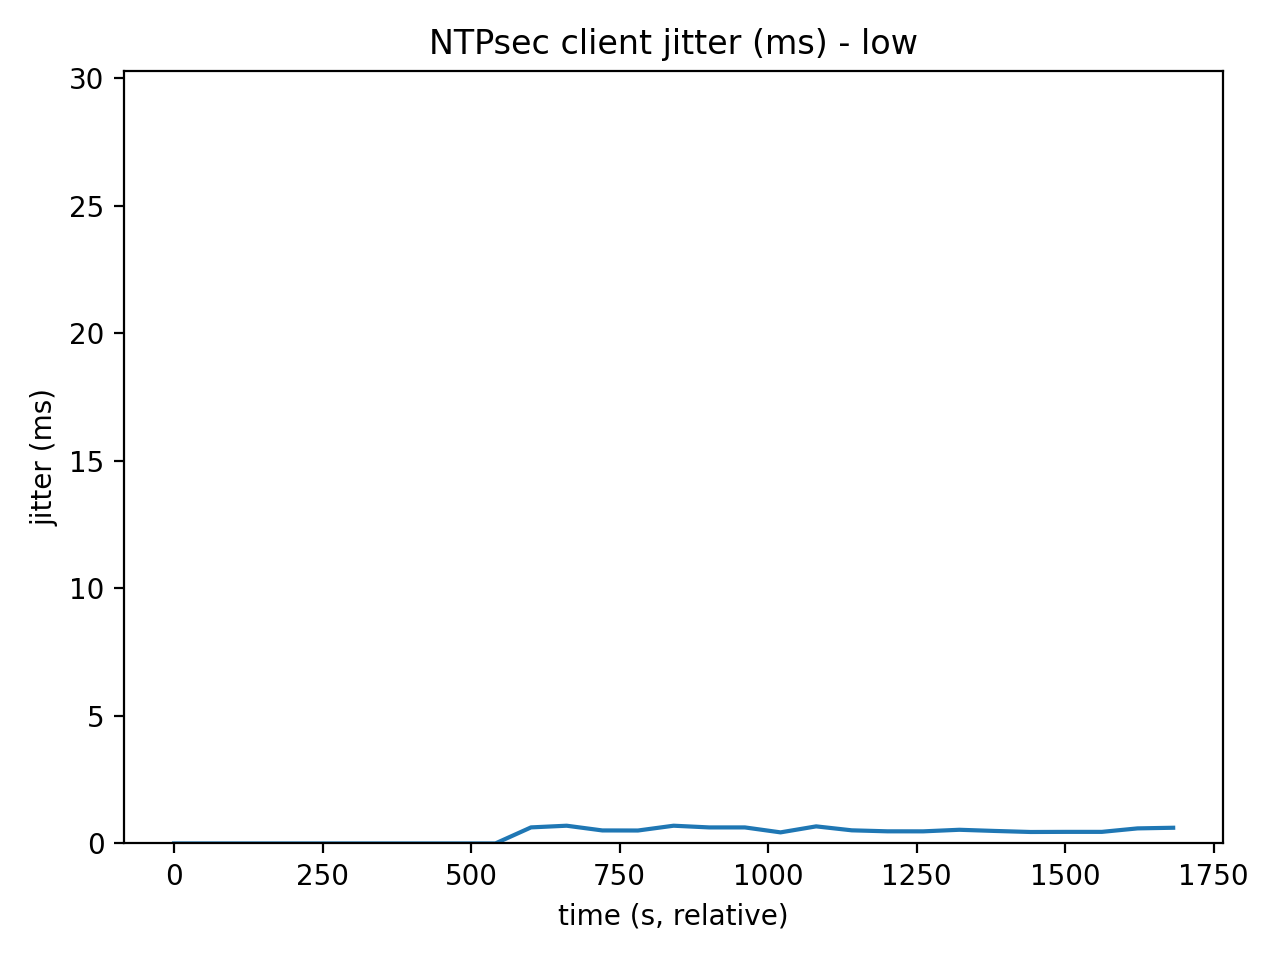
\includegraphics[width=\linewidth]{
      images/data_plots/plots_ntpsec/ntpsec_client_low_jitter_ms.png
    }
    \caption{Scenario LOW}
  \end{subfigure}
  \hfill
  \begin{subfigure}
    {0.32\textwidth}
    \centering
    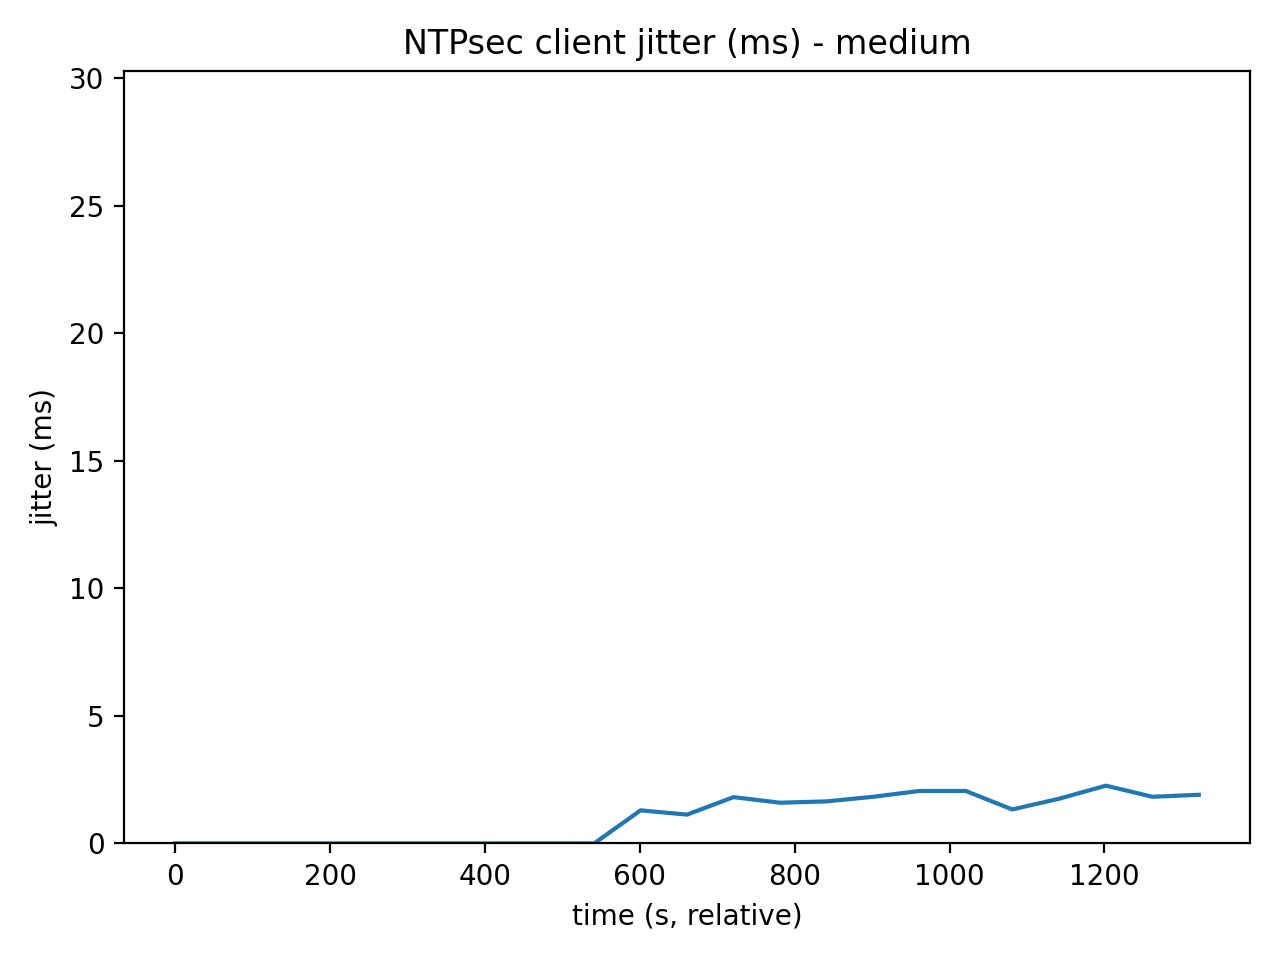
\includegraphics[width=\linewidth]{
      images/data_plots/plots_ntpsec/ntpsec_client_medium_jitter_ms.png
    }
    \caption{Scenario MEDIUM}
  \end{subfigure}
  \hfill
  \begin{subfigure}
    {0.32\textwidth}
    \centering
    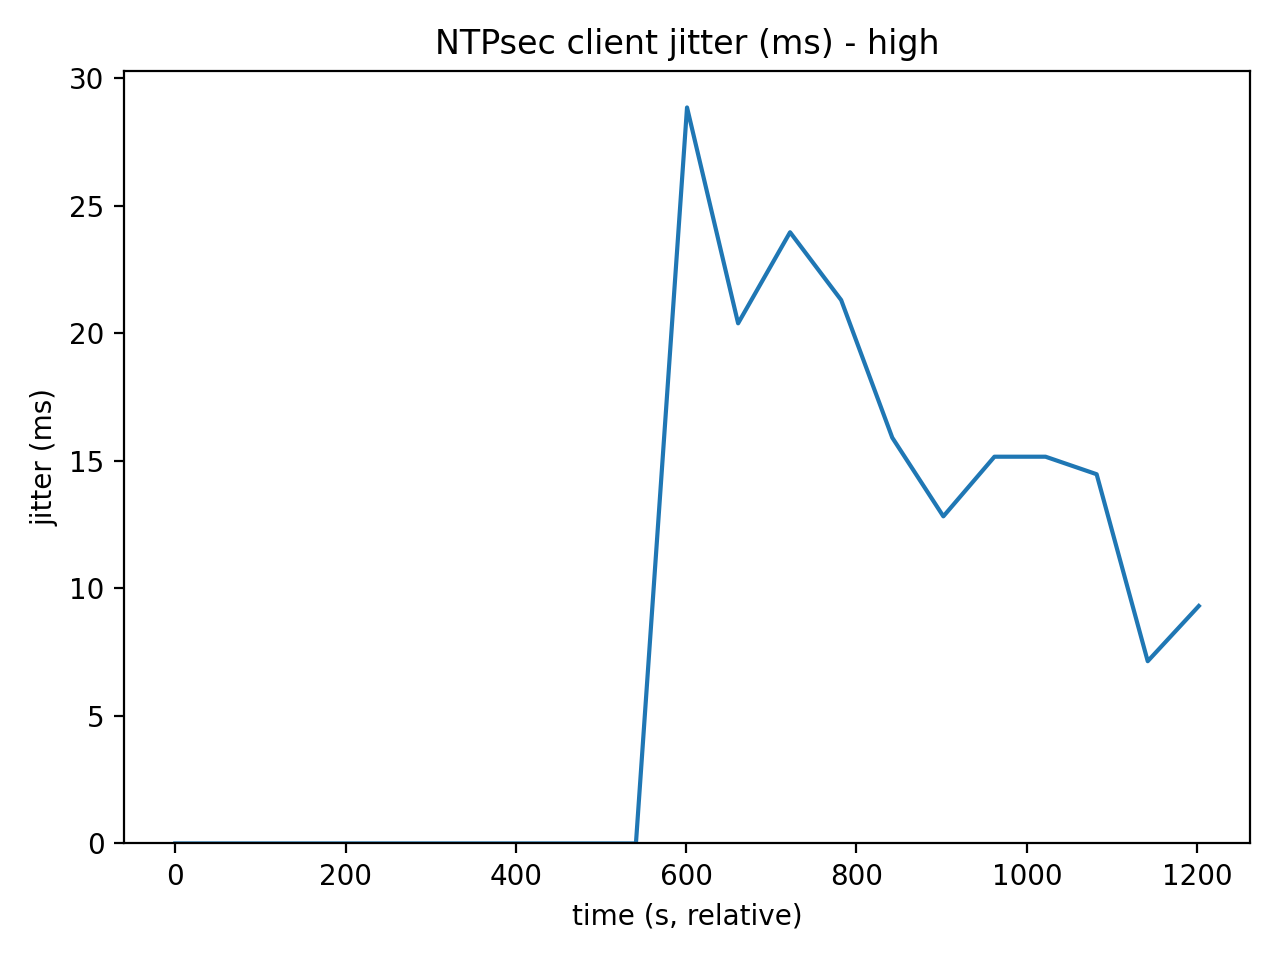
\includegraphics[width=\linewidth]{
      images/data_plots/plots_ntpsec/ntpsec_client_high_jitter_ms.png
    }
    \caption{Scenario HIGH}
  \end{subfigure}

  \caption{Comparazione della performance - nodo: \texttt{clientntp}}
  \label{fig:scenario_comparison}
\end{figure}

L’analisi del \textbf{jitter} rilevato sul nodo \texttt{clientntp} per il demone
\textbf{NTPsec} evidenzia un peggioramento progressivo della regolarità temporale
delle misurazioni al crescere della severità dello scenario di rete. Il
confronto tra i tre casi mostra infatti un incremento marcato sia del livello
della metrica sia della sua dispersione, con un passaggio netto da un regime stabile
nello scenario \texttt{low} a una condizione fortemente degradata nello scenario
\texttt{high}.

Nello scenario \texttt{low}, il jitter assume valori contenuti e si mantiene entro
una banda ristretta. Sui campioni validi si osservano una media pari a 0.5499 ms,
una mediana pari a 0.5141 ms, un primo quartile di 0.4746 ms e un terzo quartile
di 0.6281 ms, con IQR pari a 0.1535 ms. La deviazione standard è 0.0891 ms, mentre
il minimo e il massimo risultano pari rispettivamente a 0.4342 ms e 0.6951 ms.
La distribuzione appare quindi compatta e sostanzialmente regolare, senza evidenza
di valori estremi in grado di alterarne in modo significativo la struttura.

Nel caso \texttt{medium}, il jitter cresce in modo sensibile sia in termini di livello
sia in termini di dispersione. La media risulta pari a 1.7321 ms e la mediana a
1.8156 ms, con quartili pari a 1.5969 ms e 1.9073 ms e IQR di 0.3104 ms. La
deviazione standard è 0.3277 ms, il minimo è 1.1299 ms e il massimo 2.2657 ms.
Rispetto allo scenario \texttt{low}, il jitter medio risulta circa triplicato, mentre
aumentano anche l’ampiezza delle oscillazioni e la dispersione complessiva della distribuzione.

Lo scenario \texttt{high} presenta il comportamento più degradato. In questo caso
il jitter raggiunge una media pari a 16.7730 ms e una mediana pari a 15.1623 ms,
con primo quartile di 13.6496 ms, terzo quartile di 20.8481 ms e IQR pari a 7.1985
ms. La deviazione standard è 6.3757 ms, il minimo è 7.1450 ms e il massimo 28.8548
ms. Il grafico mostra una fase iniziale fortemente instabile, caratterizzata da un
picco molto elevato, seguita da una riduzione progressiva della metrica verso
valori comunque molto superiori a quelli osservati negli scenari \texttt{low} e \texttt{medium}.
La differenza tra media e mediana, insieme all’ampiezza del range, indica che la distribuzione
è influenzata da valori particolarmente elevati, pur restando nel complesso
strutturalmente collocata su livelli di forte degrado.

Nel complesso, il confronto tra i tre scenari mostra una progressione molto marcata
del jitter al crescere degli impairment di rete. La media passa da 0.5499 ms
nello scenario \texttt{low} a 1.7321 ms nel caso \texttt{medium}, fino a 16.7730 ms
nel caso \texttt{high}; analogamente, l’IQR cresce da 0.1535 ms a 0.3104 ms fino
a 7.1985 ms. Il jitter si conferma pertanto una metrica particolarmente efficace nel
mettere in evidenza l’impatto del degrado della rete sulla stabilità temporale delle
misurazioni osservate dal clientntp NTPsec.

\subsubsection{Analisi matrica: \texttt{offset}}
\begin{figure}[H]
  \centering

  \begin{subfigure}
    {0.32\textwidth}
    \centering
    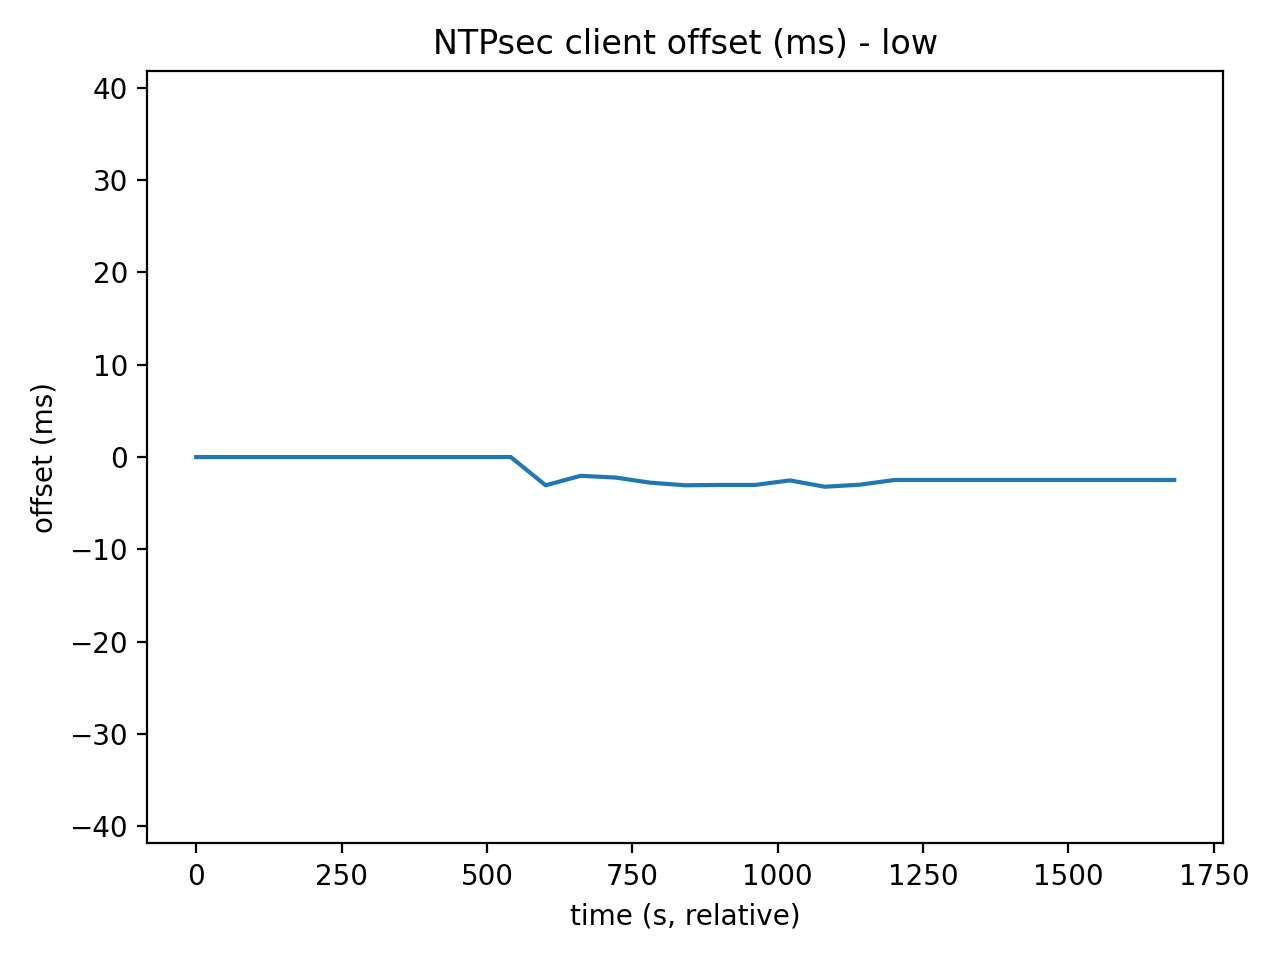
\includegraphics[width=\linewidth]{
      images/data_plots/plots_ntpsec/ntpsec_client_low_offset_ms.png
    }
    \caption{Scenario LOW}
  \end{subfigure}
  \hfill
  \begin{subfigure}
    {0.32\textwidth}
    \centering
    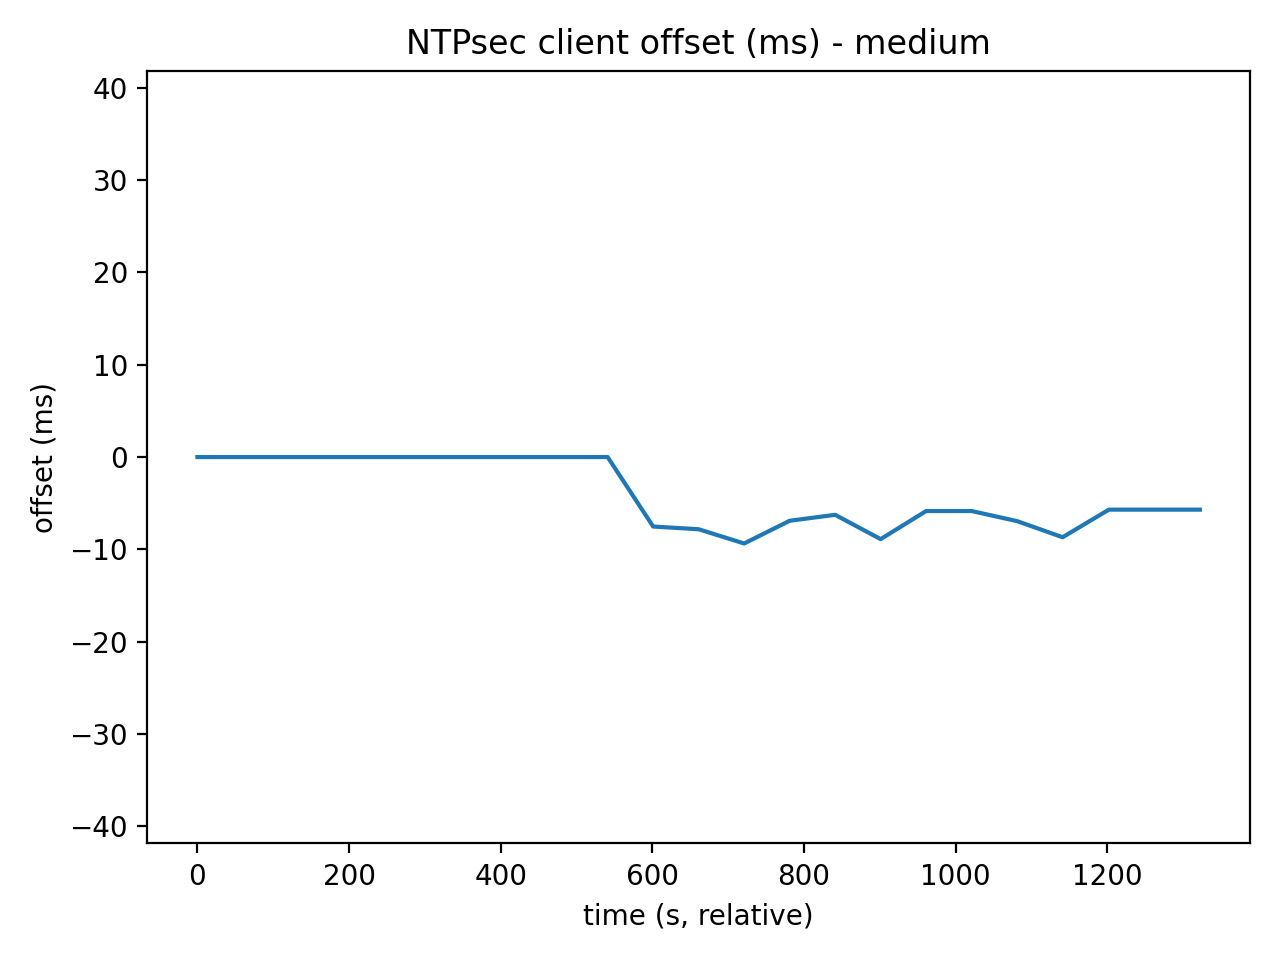
\includegraphics[width=\linewidth]{
      images/data_plots/plots_ntpsec/ntpsec_client_medium_offset_ms.png
    }
    \caption{Scenario MEDIUM}
  \end{subfigure}
  \hfill
  \begin{subfigure}
    {0.32\textwidth}
    \centering
    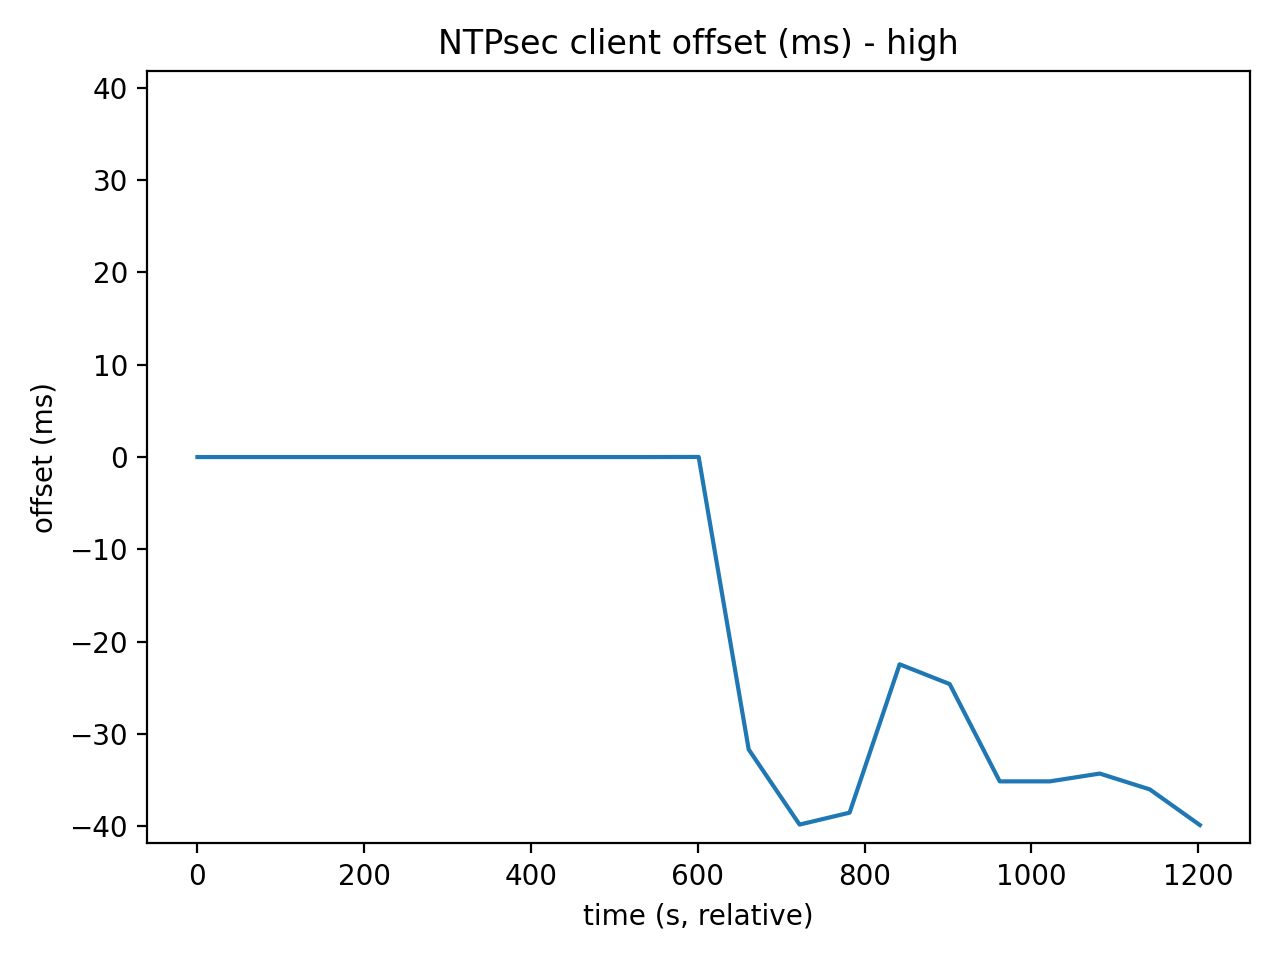
\includegraphics[width=\linewidth]{
      images/data_plots/plots_ntpsec/ntpsec_client_high_offset_ms.png
    }
    \caption{Scenario HIGH}
  \end{subfigure}

  \caption{Comparazione della performance - nodo: \texttt{clientntp}}
  \label{fig:scenario_comparison}
\end{figure}

L’analisi dell’\textbf{offset} misurato sul nodo \texttt{clientntp} per il demone
\textbf{NTPsec} evidenzia una progressiva perdita di accuratezza della
sincronizzazione al crescere della severità dello scenario di rete. Dopo la fase iniziale
di inizializzazione, in tutti e tre i casi il clientntp entra in un regime
operativo in cui l’offset assume valori sistematicamente negativi; al crescere degli
impairment, tali valori si allontanano progressivamente dallo zero e mostrano
una dispersione crescente.

Nello scenario \texttt{low}, l’offset si mantiene entro una banda relativamente
ristretta, con media pari a -2.6458 ms e mediana pari a -2.4823 ms. I quartili
sono pari a -3.0084 ms e -2.4823 ms, con IQR di 0.5261 ms. Il minimo e il
massimo risultano rispettivamente pari a -3.2148 ms e -2.0321 ms, mentre la deviazione
standard è 0.3248 ms. Il grafico mostra un andamento regolare e stabile, collocato
attorno a valori moderatamente negativi, indicativo di una sincronizzazione
ancora relativamente accurata.

Nel caso \texttt{medium}, l’offset si sposta in modo netto verso valori più
negativi. La media risulta pari a -7.0136 ms e la mediana a -6.9026 ms, con
quartili pari a -7.8200 ms e -5.8483 ms e IQR di 1.9717 ms. Il minimo è -9.3643
ms, il massimo -5.6966 ms e la deviazione standard 1.3313 ms. Rispetto allo scenario
\texttt{low}, il valore tipico dell’offset si allontana quindi in modo sensibile dallo
zero, mentre cresce anche la dispersione complessiva della metrica.

Lo scenario \texttt{high} presenta il comportamento più degradato. In questo
caso l’offset assume media pari a -30.6788 ms e mediana pari a -35.1341 ms, con quartili
di -37.2646 ms e -28.1322 ms e IQR di 9.1325 ms. Il minimo osservato è -39.8648 ms,
mentre il massimo è 0.0131 ms. Il grafico mostra che, dopo un primo campione
prossimo allo zero, la serie entra rapidamente in un regime fortemente negativo,
senza più tornare verso i livelli osservati negli scenari precedenti. La differenza
tra media e mediana indica che la distribuzione è influenzata da tale campione iniziale,
mentre la mediana descrive più fedelmente il livello tipico dell’offset in
regime, pari a circa -35 ms.

Nel complesso, il confronto tra i tre scenari mostra una progressione molto marcata
dell’offset in valore assoluto: la media passa da -2.6458 ms nello scenario \texttt{low}
a -7.0136 ms nel caso \texttt{medium}, fino a -30.6788 ms nel caso \texttt{high};
analogamente, l’IQR cresce da 0.5261 ms a 1.9717 ms fino a 9.1325 ms. L’offset
si conferma pertanto una metrica particolarmente efficace nel mettere in
evidenza l’impatto del degrado della rete sull’accuratezza e sulla stabilità del
processo di sincronizzazione del clientntp NTPsec.

\subsection{\texttt{boundary}}
Nel caso del nodo \texttt{boundary}, l’interpretazione dei risultati richiede
una precisazione preliminare. A differenza di quanto osservato sul nodo \texttt{clientntp},
gli impairment di rete introdotti mediante \texttt{NETEM} non agiscono
direttamente sul collegamento \texttt{upstream} tra il nodo \texttt{boundary} e
il nodo di riferimento, bensì sul ramo \texttt{downstream} tra \texttt{boundary} e
\texttt{clientntp}. Ne consegue che le metriche rilevate sul \texttt{boundary}
non dovrebbero, in linea teorica, risentire in modo marcato del degrado
introdotto nei tre scenari sperimentali, o comunque non con la stessa intensità osservata
nel caso del clientntp.

L’analisi delle metriche del nodo \texttt{boundary} è pertanto orientata
principalmente a verificare la coerenza tra tale aspettativa teorica e i dati
effettivamente osservati. In particolare, il confronto tra scenari è finalizzato
a stabilire se le eventuali differenze rilevate siano effettivamente contenute, come
atteso, oppure se emergano variazioni non trascurabili che possano suggerire
effetti indiretti del degrado di rete sul comportamento del nodo.

Va inoltre considerato che il tempo di ingresso nel regime operativo può
differire rispetto a quello osservato sul nodo \texttt{clientntp}. Tale aspetto
viene tenuto in considerazione nell’interpretazione dei risultati, pur non costituendo,
di per sé, l’oggetto principale del confronto tra scenari.

\subsubsection{Analisi metriche: \texttt{delay, jitter, offset}}
\begin{figure}[H]
  \centering

  \begin{subfigure}
    {0.32\textwidth}
    \centering
    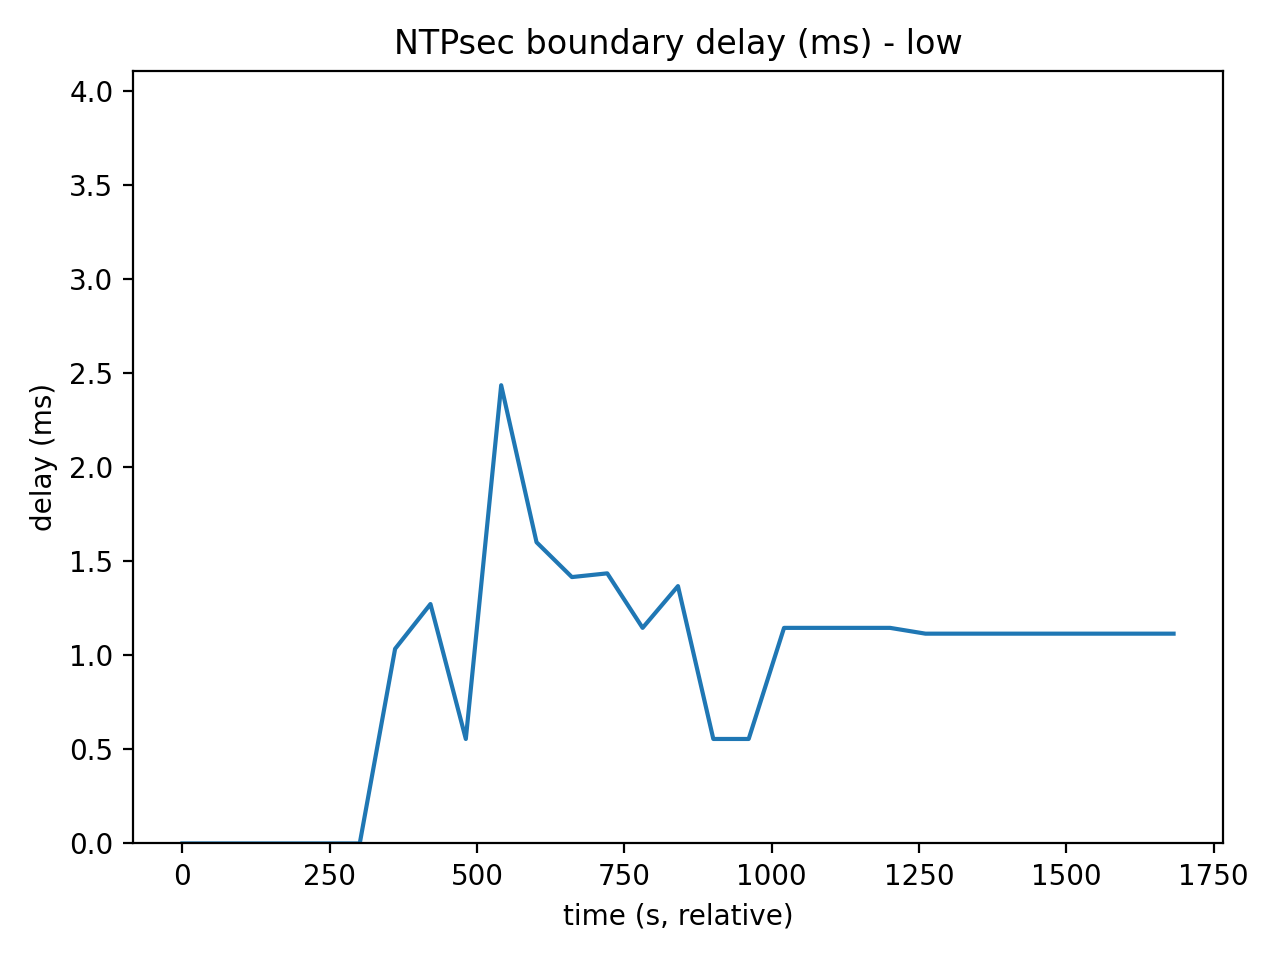
\includegraphics[width=\linewidth]{
      images/data_plots/plots_ntpsec/ntpsec_boundary_low_delay_ms.png
    }
    \caption{Scenario LOW}
  \end{subfigure}
  \hfill
  \begin{subfigure}
    {0.32\textwidth}
    \centering
    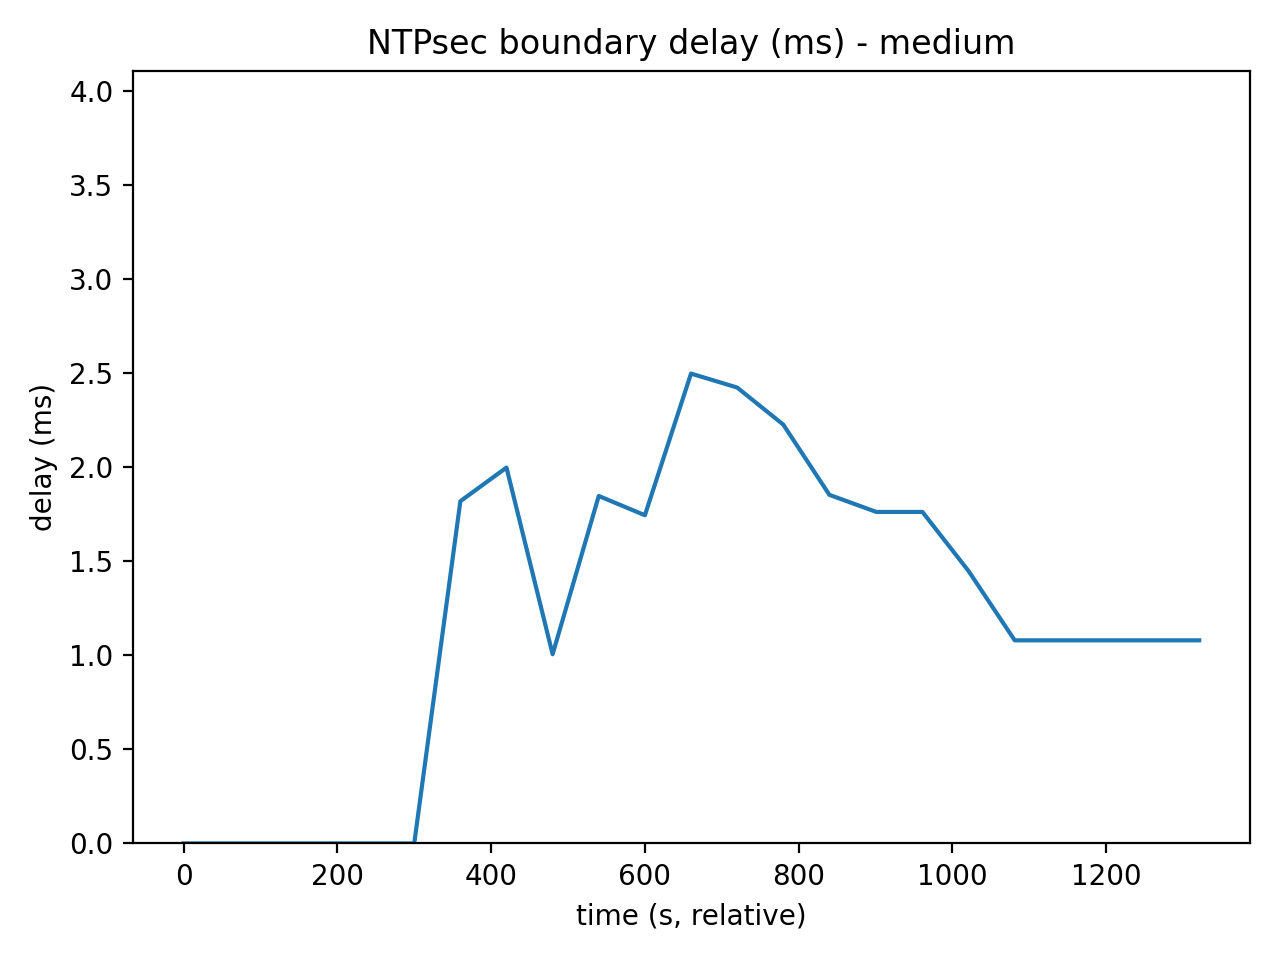
\includegraphics[width=\linewidth]{
      images/data_plots/plots_ntpsec/ntpsec_boundary_medium_delay_ms.png
    }
    \caption{Scenario MEDIUM}
  \end{subfigure}
  \hfill
  \begin{subfigure}
    {0.32\textwidth}
    \centering
    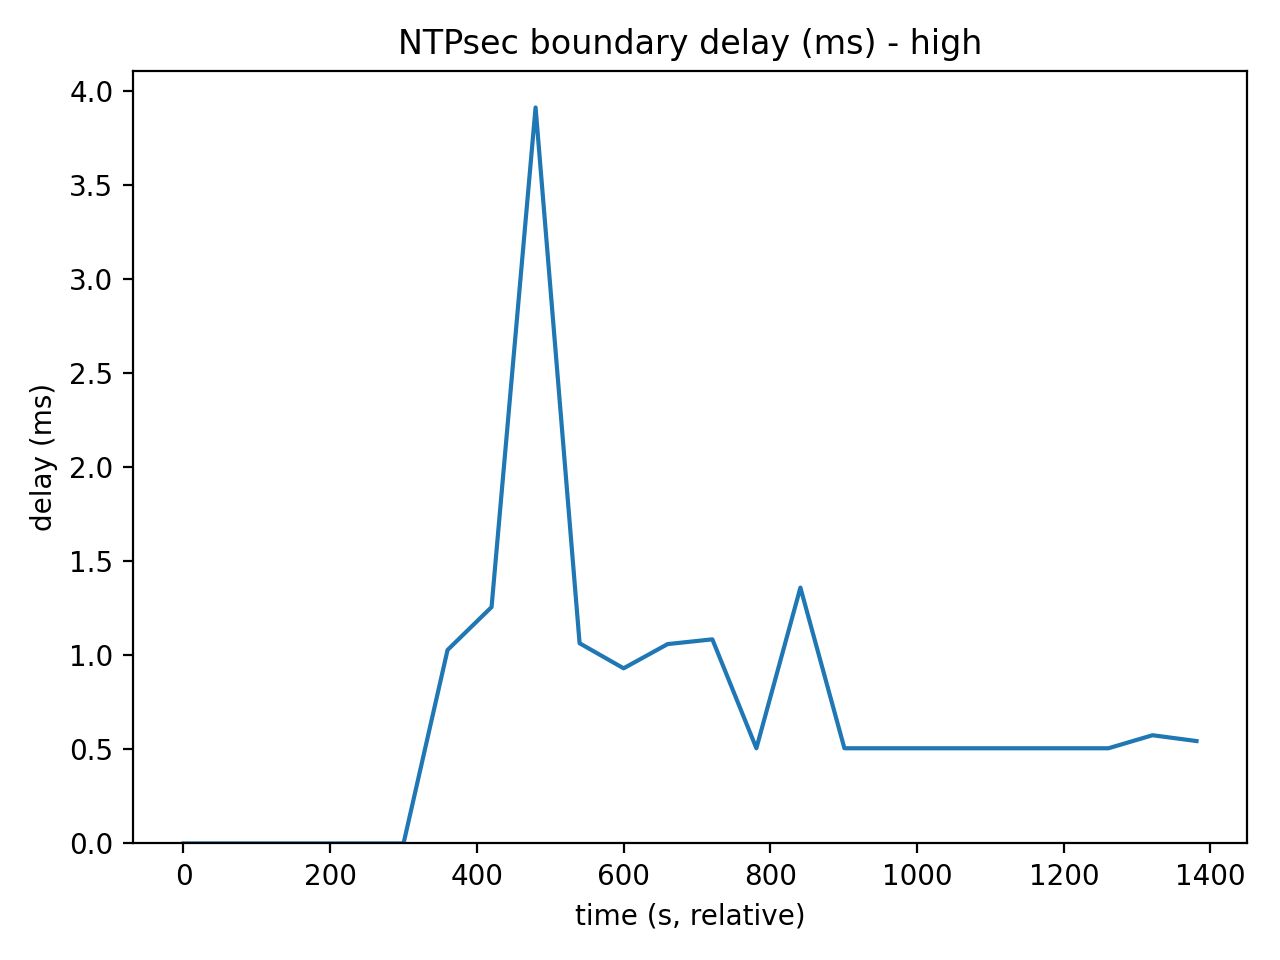
\includegraphics[width=\linewidth]{
      images/data_plots/plots_ntpsec/ntpsec_boundary_high_delay_ms.png
    }
    \caption{Scenario HIGH}
  \end{subfigure}

  \caption{Comparazione della performance - nodo: \texttt{boundary} metrica: \texttt{delay}}
  \label{fig:scenario_comparison}
\end{figure}

\begin{figure}[H]
  \centering

  \begin{subfigure}
    {0.32\textwidth}
    \centering
    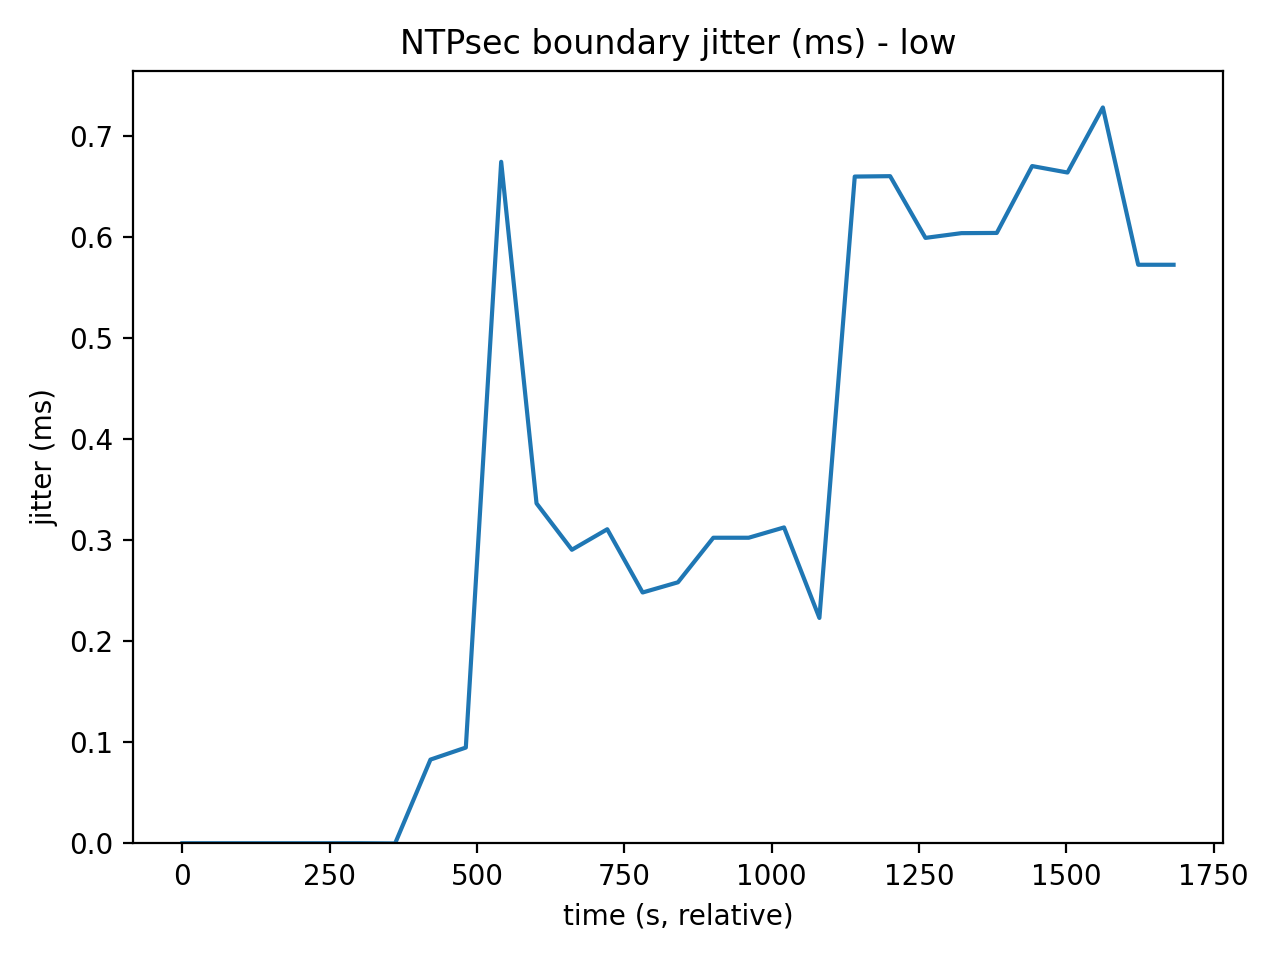
\includegraphics[width=\linewidth]{
      images/data_plots/plots_ntpsec/ntpsec_boundary_low_jitter_ms.png
    }
    \caption{Scenario LOW}
  \end{subfigure}
  \hfill
  \begin{subfigure}
    {0.32\textwidth}
    \centering
    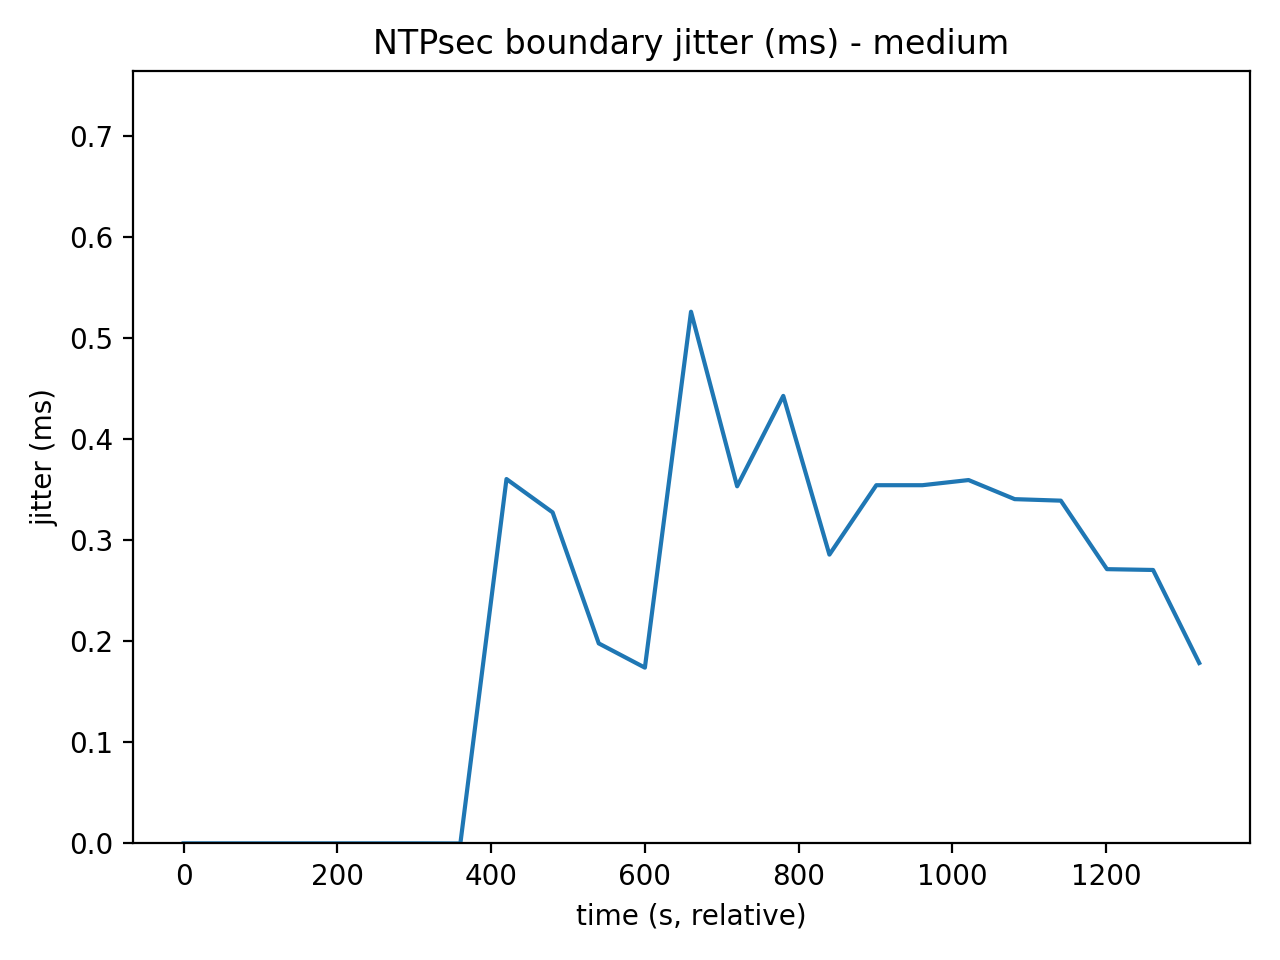
\includegraphics[width=\linewidth]{
      images/data_plots/plots_ntpsec/ntpsec_boundary_medium_jitter_ms.png
    }
    \caption{Scenario MEDIUM}
  \end{subfigure}
  \hfill
  \begin{subfigure}
    {0.32\textwidth}
    \centering
    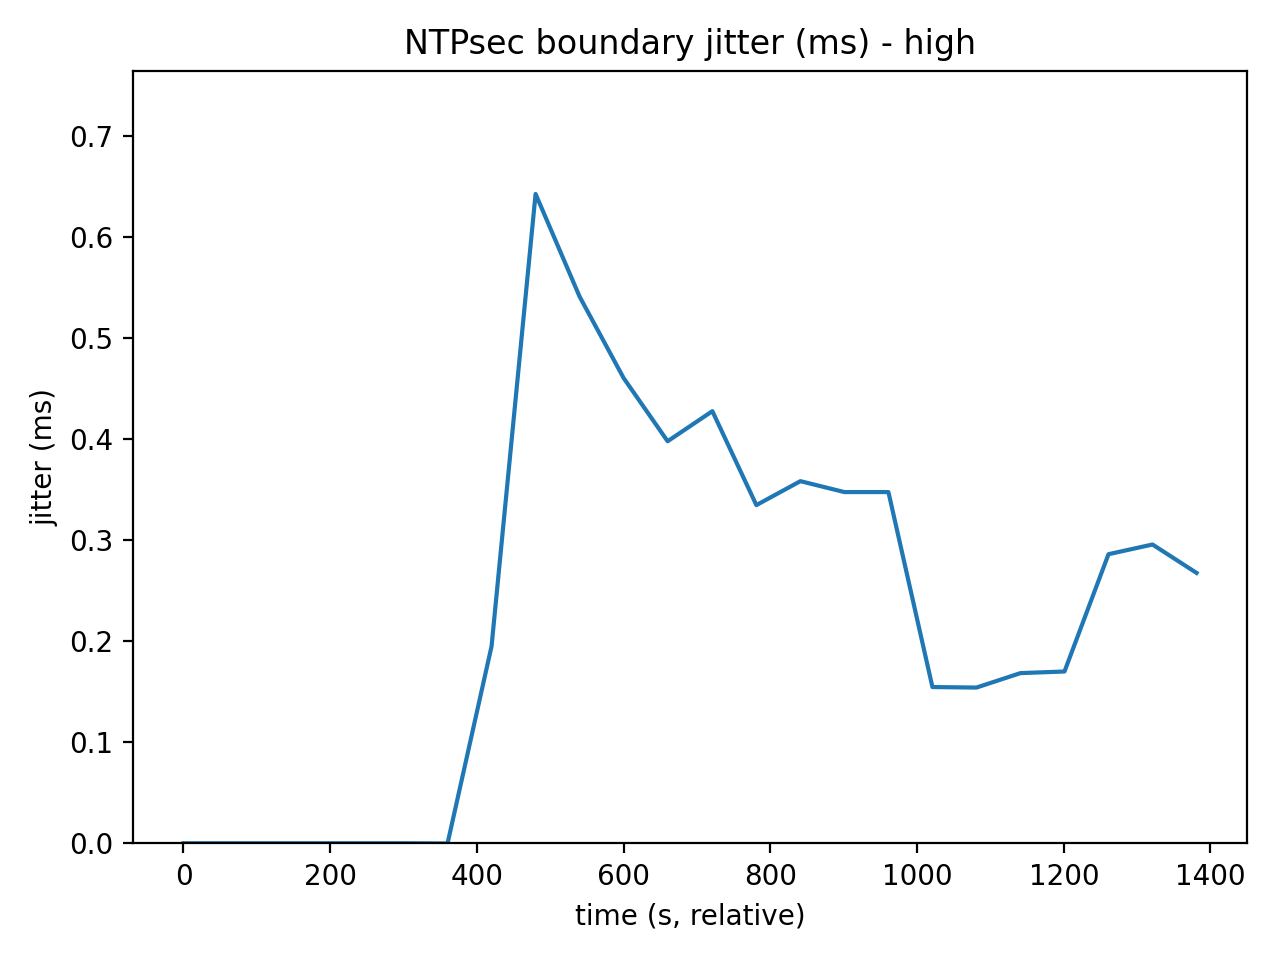
\includegraphics[width=\linewidth]{
      images/data_plots/plots_ntpsec/ntpsec_boundary_high_jitter_ms.png
    }
    \caption{Scenario HIGH}
  \end{subfigure}

  \caption{Comparazione della performance - nodo: \texttt{boundary} metrica: \texttt{jitter}}
  \label{fig:scenario_comparison}
\end{figure}

\begin{figure}[H]
  \centering

  \begin{subfigure}
    {0.32\textwidth}
    \centering
    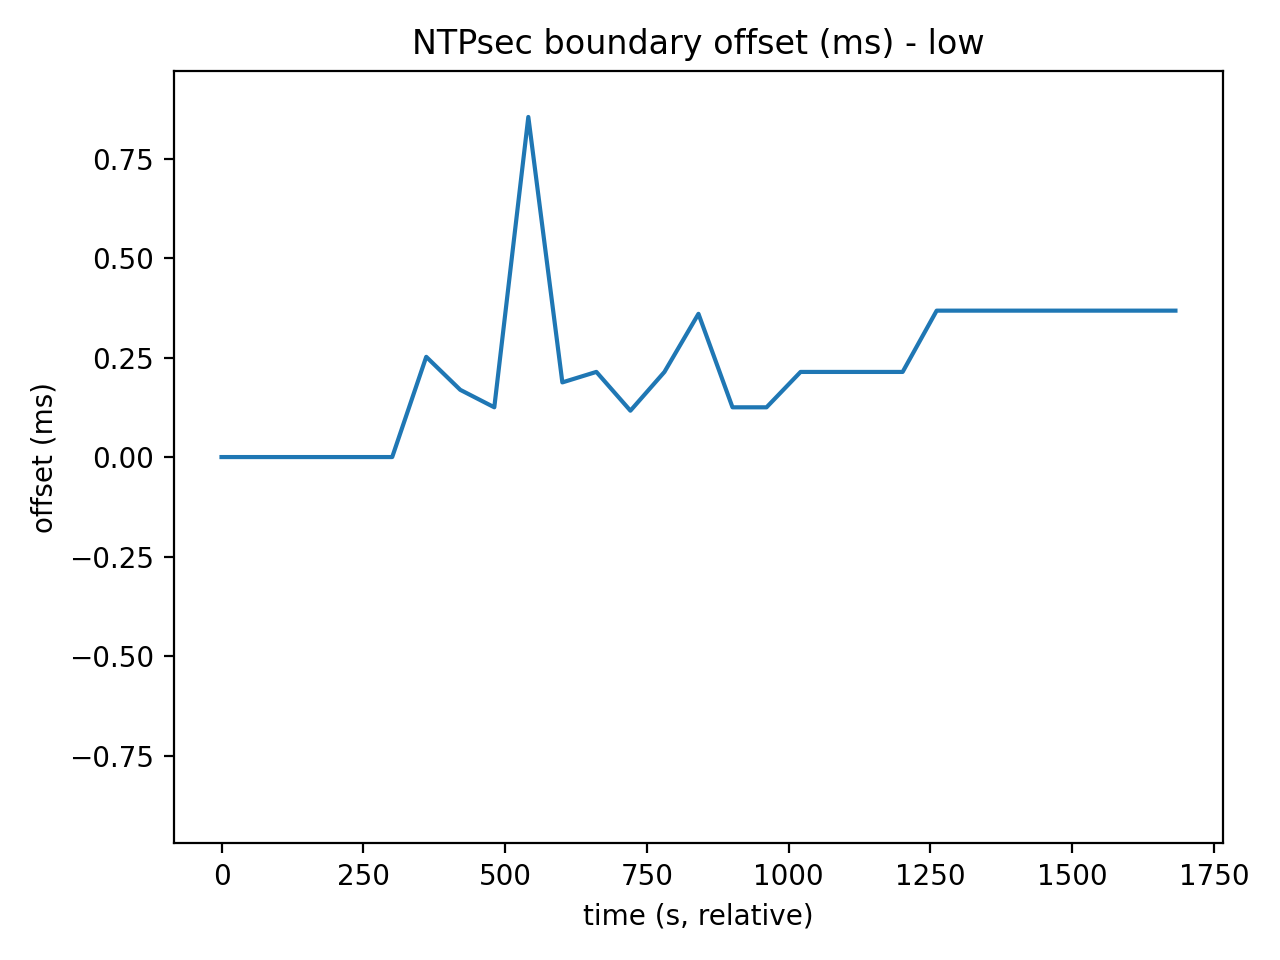
\includegraphics[width=\linewidth]{
      images/data_plots/plots_ntpsec/ntpsec_boundary_low_offset_ms.png
    }
    \caption{Scenario LOW}
  \end{subfigure}
  \hfill
  \begin{subfigure}
    {0.32\textwidth}
    \centering
    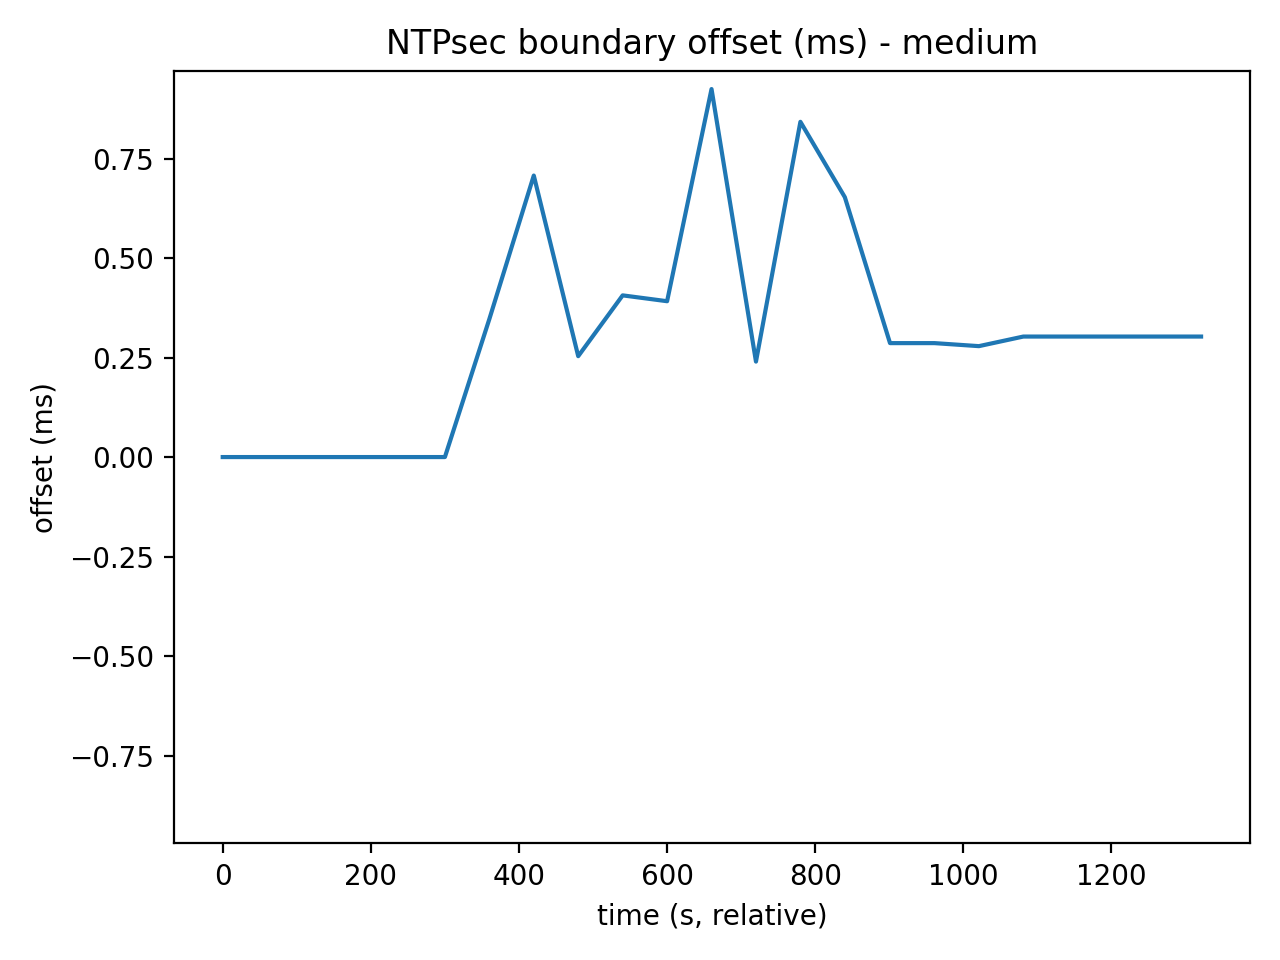
\includegraphics[width=\linewidth]{
      images/data_plots/plots_ntpsec/ntpsec_boundary_medium_offset_ms.png
    }
    \caption{Scenario MEDIUM}
  \end{subfigure}
  \hfill
  \begin{subfigure}
    {0.32\textwidth}
    \centering
    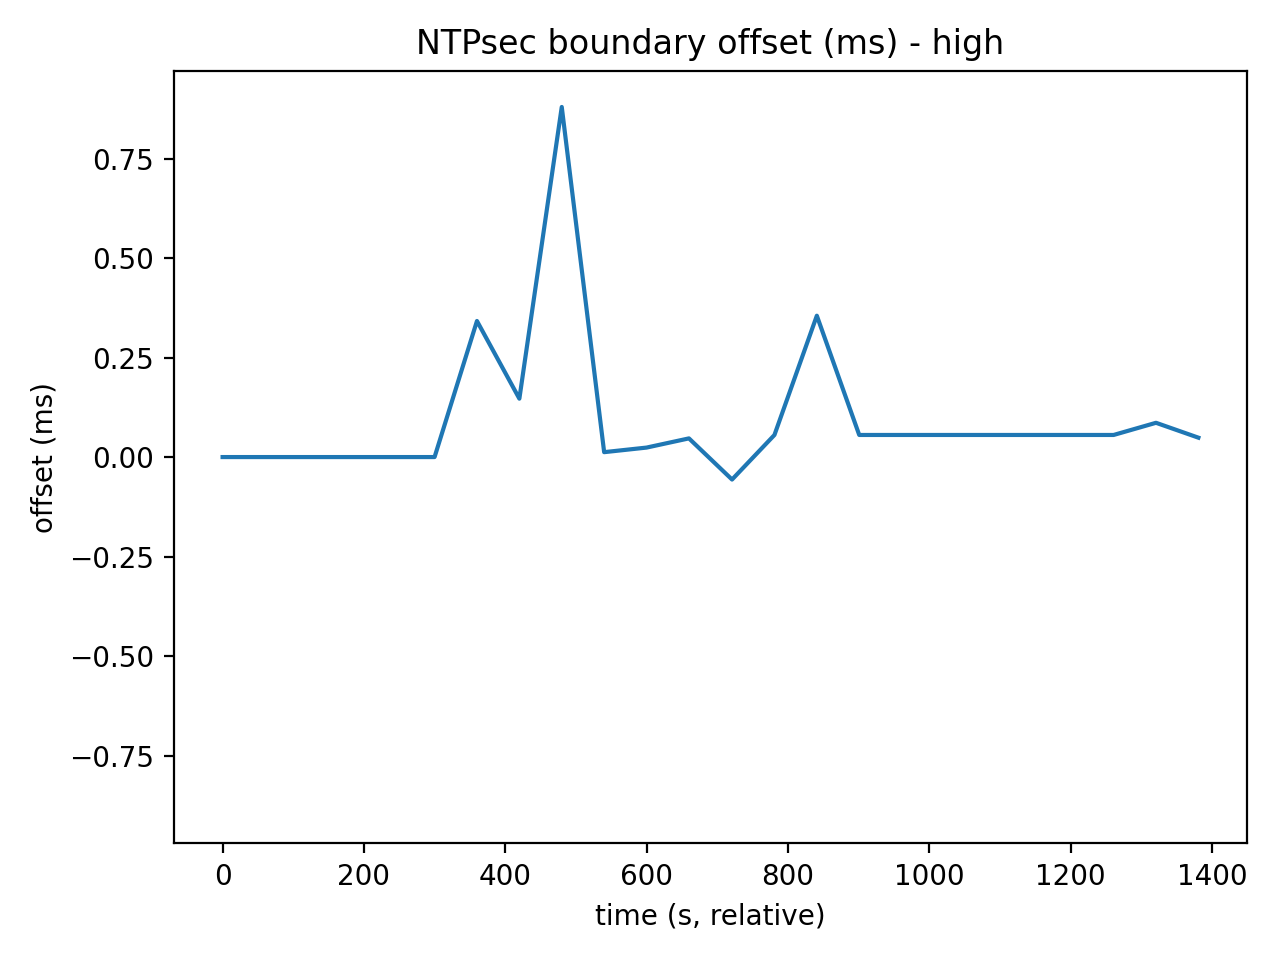
\includegraphics[width=\linewidth]{
      images/data_plots/plots_ntpsec/ntpsec_boundary_high_offset_ms.png
    }
    \caption{Scenario HIGH}
  \end{subfigure}

  \caption{Comparazione della performance - nodo: \texttt{boundary} metrica: \texttt{offset}}
  \label{fig:scenario_comparison}
\end{figure}

Nel caso del nodo \texttt{boundary}, il confronto tra scenari non evidenzia un
degrado sistematico e paragonabile a quello osservato precedentemente nel
\texttt{clientntp}. Tale risultato è coerente con la configurazione sperimentale
adottata: gli impairment di rete introdotti mediante \texttt{NETEM} agiscono
infatti sul ramo \texttt{downstream} tra \texttt{boundary} e \texttt{clientntp},
mentre le metriche qui considerate descrivono il comportamento del nodo \texttt{boundary}
rispetto al proprio riferimento \texttt{upstream} con il nodo \texttt{servergm},
non direttamente soggetto al degrado configurato.

Un primo elemento coerente con tale interpretazione riguarda il tempo di
ingresso nel regime operativo. Nei tre scenari, il nodo \texttt{boundary} raggiunge
infatti i primi campioni validi attorno a $540$–$541$ secondi, quindi in
anticipo rispetto al nodo \texttt{clientntp}, per il quale i campioni validi
iniziano a circa $601$ secondi. Ciò suggerisce che il processo di selezione e stabilizzazione
della sorgente risulta meno penalizzato sul ramo \texttt{upstream} osservato dal
\texttt{boundary}.

Anche l’analisi delle singole metriche conferma l’assenza di un degrado netto al crescere
della severità dello scenario. Il \texttt{delay} medio passa da 1.2016 ms nello scenario
\texttt{low} a 1.6412 ms nel caso \texttt{medium}, per poi ridursi a 0.7116 ms
nello scenario \texttt{high}. L’\texttt{offset} medio rimane in tutti i casi
contenuto e prossimo allo zero, con valori pari a 0.2998 ms, 0.4159 ms e 0.0640
ms rispettivamente nei tre scenari. Analogamente, il \texttt{jitter} resta su livelli
bassi e relativamente stabili, assumendo valori medi pari a 0.4799 ms nel caso
\texttt{low}, 0.3179 ms nel caso \texttt{medium} e 0.3143 ms nel caso \texttt{high}.

Nel complesso, le differenze osservate tra scenari risultano moderate e non seguono
una progressione monotona con l’aumentare degli impairment. Questo comportamento
suggerisce che il nodo \texttt{boundary} mantiene una condizione di sincronizzazione
sostanzialmente stabile rispetto al proprio collegamento di riferimento, e che
l’effetto del degrado introdotto sulla rete si manifesta in modo molto marcato
solamente sul nodo \texttt{clientntp} che non sul \texttt{boundary}. Le variazioni
residue osservate nelle metriche del \texttt{boundary} possono pertanto essere
interpretate come oscillazioni contenute del processo di sincronizzazione, piuttosto
che come evidenza di un deterioramento strutturale legato allo scenario sperimentale.